\documentclass[norsk,a4paper,12pt]{article}
\usepackage[utf8]{inputenc}
\usepackage{graphicx} %for å inkludere grafikk
\usepackage{verbatim} %for å inkludere filer med tegn LaTeX ikke liker
\usepackage{tabularx}
\usepackage{booktabs}
\usepackage{amsmath}
\usepackage{float}
\usepackage{color}
\usepackage{listings}
\usepackage{hyperref}
\usepackage{amsmath}

\lstset{language=c++}
\lstset{basicstyle=\small}
\lstset{backgroundcolor=\color{white}}
\lstset{frame=single}
\lstset{stringstyle=\ttfamily}
\lstset{keywordstyle=\color{red}\bfseries}
\lstset{commentstyle=\itshape\color{blue}}
\lstset{showspaces=false}
\lstset{showstringspaces=false}
\lstset{showtabs=false}
\lstset{breaklines}
\lstset{postbreak=\raisebox{0ex}[0ex][0ex]{\ensuremath{\color{red}\hookrightarrow\space}}}
\usepackage{titlesec}

\setcounter{secnumdepth}{4}

\titleformat{\paragraph}
{\normalfont\normalsize\bfseries}{\theparagraph}{1em}{}
\titlespacing*{\paragraph}
{0pt}{3.25ex plus 1ex minus .2ex}{1.5ex plus .2ex}


\title{FYS4411 - Computational Physics II\\\vspace{2mm} \Large{Project 1}}
\author{\large Dorthea Gjestvang\\ Even Marius Nordhagen}
\date\today
\begin{document}

\maketitle
\begin{abstract}
Write the abstract here
\par 

\end{abstract}


\begin{itemize}
\item Github repository containing programs and results are in: \url{https://github.com/evenmn/FYS4411/tree/master/Project%201}
\end{itemize}


\section{Introduction}
Introduction

\section{Theory}
We study a system of $N$ bosons trapped in a harmonic oscillator with the Hamiltonian given by 
\begin{equation}
\hat{H}=\sum_i^N\bigg(-\frac{\hbar^2}{2m}\nabla_i^2+V_{ext}(\vec{r}_i)\bigg)+\sum_{i<j}^NV_{int}(\vec{r}_i,\vec{r}_j)
\end{equation}
with $V_{ext}$ as the external potential, which is the harmonic oscillator potential,
and $V_{int}$ as the interaction term, which can be ignored when developing the benchmarks. 

The wavefunction is on the form 
\begin{equation}
\Psi_T(\vec{r}_1, \vec{r}_2, ..., \vec{r}_N, \alpha, \beta)=\prod_i^Ng(\alpha, \beta, \vec{r}_i)\prod_{i<j}f(a,r_{ij})
\end{equation}
where $r_{ij}=|\vec{r}_i-\vec{r}_j|$ and $g$ is assumed to be an exponential
\begin{equation}
g(\alpha, \beta, \vec{r}_i)=\exp[-\alpha(x_i^2+y_i^2+\beta z_i^2)]
\end{equation}
which is practical since
\begin{equation}
\prod_i^Ng(\alpha, \beta, \vec{r}_i)=\exp[-\alpha(x_1^2+y_1^2+\beta z_1^2+\cdots x_N^2+y_N^2+\beta z_N^2)].
\end{equation}
$\alpha$ is a variational parameter that we later use to find the energy minimum, and $\beta$ is a constant. The $f$ presented above is the correlation wave function, which is 
\begin{equation}
f(a,r_{ij})=
\begin{cases} 
   0 & r_{ij} \leq a \\
   \left(1-\frac{a}{r_{ij}}\right) & r_{ij} > a.
\end{cases}
\end{equation}
The first case we will take into account, is when $a=0$, and one might observe that $f=1$ then. Anyway, ...

We want to calculate the local energy as a function of $\alpha$, and then use Variational Monte Carlo (VMC) described in section \ref{VMC}. For the non-interacting case, the analytical expression is well-known and given by
\begin{equation}
E = \hbar\omega(n + 1/2)
\end{equation}
where $n$ is the total number of free dimensions, which gonna be an useful benchmark. The local energy is
\begin{equation}
E_L(\vec{r})=\frac{1}{\Psi_T(\vec{r})}\hat{H}\Psi_T(\vec{r})
\end{equation}
which gives the following results considering $a=0$:

INSERT ANALYTICAL EXPRESSIONS FROM A

For $a\neq0$ it gets rather more complicated, because we need to deal with the correction wave function as well. By defining
\begin{equation}
f(a, r_{ij})=\exp{\bigg(\sum_{i<j}u(r_{ij})\bigg)}
\end{equation}
and doing a change of variables
\begin{equation}
\frac{\partial}{\partial r_k}=\frac{\partial}{\partial r_k}\frac{\partial r_{kj}}{\partial r_{kj}}=\frac{\partial r_{kj}}{\partial r_k}\frac{\partial}{\partial r_{kj}}=\frac{(r_k-r_j)}{r_{kj}}\frac{\partial}{\partial r_{kj}}
\end{equation}
one will end up with
\begin{align}
E_L=\sum_k\Bigg(-\frac{1}{2}\bigg(&4\alpha^2\Big(x_k^2+y_k^2+\beta^2z_k^2-\frac{1}{\alpha}-\frac{\beta}{2\alpha}\Big)\notag\\
&-4\alpha\sum_{j\neq k}(x_k, y_k, \beta z_k)\frac{(\vec{r}_k-\vec{r}_j)}{r_{kj}}u'(r_{kj})\\
&+\sum_{ij\neq k}\frac{(\vec{r}_k-\vec{r}_j)(\vec{r}_k-\vec{r}_i)}{r_{ki}r_{kj}}u'(r_{ki})u'(r_{kj})\notag\\
&+\sum_{j\neq k}\Big(u''(r_{kj})+\frac{2}{r_{kj}}u'(r_{kj})\Big)\bigg)+V_{ext}(\vec{r}_k)\Bigg).\notag
\end{align}
This is not a pretty expression, but .. We could also split up the local energy expression 
\begin{equation}
E_{L,i}=-\frac{\hbar^2}{2m}\frac{\nabla_i^2\Psi_T}{\Psi_T}+V_{ext}(\vec{r}_i)=E_{k,i}+E_{p,i}
\end{equation}
and calculate the local energy with a numerical approach where the second derivative can be approximated by the three-point formula:
\begin{equation}
f''(x)\simeq\frac{f(x+h)-2f(x)+f(x-h)}{h^2}.
\end{equation}
In our case the position is a three dimensional vector, so we need to handle each dimension separately. However, in section \ref{CPU}, the CPU time for the analytical and numerical approach are compared. 


\section{Methods}
\subsection{Variational Monte Carlo}\label{VMC}
Variational Monte Carlo (VMC) is a widely used method for approximating the ground state of a quantum system. The method is based on Markov chains, and move a particle (or a set of particles) one step for each cycle, i.e.
\begin{equation}
\vec{R}_{new} = \vec{R} + r\cdot \text{step}
\end{equation}
Both the direction and the change in position are randomly chosen, so with a plain VMC implementation the particles will move randomly and independently of each other. We are going to use the Metropolis algorithm in addition to the VMC, which accepts or rejects moves based on the probability ratio between the old and the new position. This makes the system approach the most likely state, and the idea is that after a certain number of cycles the system will be in the most likely state. 

\subsection{Metropolis Algorithm}
As mentioned above the task of the Metropolis algorithm is to move the system against the most likely state. The original algorithm, here named brute force, is the simplest one, and does not deal with the transition probabilities. The modified Metropolis-Hastings algorithm includes, on the other hand, the transition probabilities and will be slightly more time consuming per cycle. We expect the latter to converge faster to the most likely state. 

The foundation of the Metropolis algorithm is that the probability for a system to undergo a transition from state $i$ to state $j$ is given by the transition probability multiplied by the acceptance probability
\begin{equation}
W_{i\rightarrow j} = T_{i \rightarrow j}\cdot A_{i \rightarrow j}
\end{equation}
where $T_{i \rightarrow j}$ is the transition probability and $A_{i \rightarrow j}$ is the acceptance probability. Built on this, the probability for being in a state $i$ at time (step) $n$ is
\begin{equation}
P_i^{(n)} = \sum_j\bigg[P_j^{(n-1)}T_{j \rightarrow i}A_{j \rightarrow i} + P_i^{(n-1)}T_{i \rightarrow j}(1-A_{i \rightarrow j})\bigg]
\end{equation}
since this can happend in two ways. One can start in this state $i$ at time $n-1$ and be rejected or one can start in another state $j$ at time $n-1$ and complete an accepted move to state $i$. In fact $\sum_j T_{i \rightarrow j} =1$, so we can rewrite this as 
\begin{equation}
P_i^{(n)} = P_i^{(n-1)} + \sum_j\bigg[P_j^{(n-1)}T_{j \rightarrow i}A_{j \rightarrow i} - P_i^{(n-1)}T_{i \rightarrow j}A_{i \rightarrow j}\bigg].
\end{equation}
When the times goes to infinity, the system will approach the most likely state and we will have $P_i^{(n)} = p_i$, which requires
\begin{equation}
\sum_j\bigg[p_jT_{j \rightarrow i}A_{j \rightarrow i} - p_iT_{i \rightarrow j}A_{i \rightarrow j}\bigg]=0.
\end{equation}
Rearranging, we obtain a quite useful results
\begin{equation}
\frac{A_{j\rightarrow i}}{A_{i\rightarrow j}}=\frac{p_iT_{i\rightarrow j}}{p_jT_{j\rightarrow i}}
\end{equation}

\subsubsection{Brute force}
In the brute force Metropolis algorithm we want to check if the new position is more likely than the current position, and for that we calculate the probabilities $P(\vec{R})=|\Psi_T(\vec{R})|^2$ for both positions. We get rid off the transition probabilities setting $T_{i\rightarrow j}=T_{j\rightarrow i}$, and then end up with the plain ratio
\begin{equation}
w=\frac{P(\vec{R}_{new})}{P(\vec{R})}=\frac{|\Psi_T(\vec{R}_{new})|^2}{|\Psi_T(\vec{R})|^2}.
\end{equation}
$w$ will be larger than one if the new position is more likely than the current, and smaller than one if the current position is more likely than the new one. Metropolis handle this by accepting if the ratio $w$ is larger than a random number $r$ in the interval $[0,1]$, and rejecting if not:
\begin{equation}
\text{New position: }
\begin{cases} 
   \text{accept} & \text{if}\quad w > r \\
   \text{reject} & \text{if}\quad w \leq r.
\end{cases}
\end{equation}

\subsubsection{Importance sampling}
The important sampling technique is often refered to as Metropolis-Hastings algorithm. The approach is the same as for the brute force Metropolis algorithm, but we will end ut with a slightly more complicated acceptation criteria. To understand the details, we need to begin with the Fokker-Planck equation, which describes the time-evolution of the probability density function $P(R,t)$. In one dimension it reads
\begin{equation}
\frac{\partial P(R,t)}{\partial t} = D\frac{\partial}{\partial R}\bigg(\frac{\partial}{\partial R} - F\bigg)P(R,t).
\end{equation}
where $F$ is the drift force and $D$ is the diffusion coefficient. Even though the probability density function can give a lot of useful information, an equation describing the motion of a such particle would be more appropriate for our purposes. Fortunately this equation exists, and satisfies the Fokker-Planck equation. The Langevin equation is given by
\begin{equation}
\frac{\partial R(t)}{\partial t}=DF(R(t)) + \eta
\end{equation}
where $\eta$ can be considered as a random variable. One can solve this differetial equation by applying the forward Euler method and introducing gaussian variables $\xi$
\begin{equation}
R_{new} = R + DF(R)\Delta t + \xi\sqrt{\Delta t}
\end{equation}
which will be used to update the position. Moreover we also need to update the acceptance criteria since we no longer ignore the transition probabilities. With the Fokker-Planck equation as base, the transition probabilities are given by Green's function
\begin{align}
T_{R\rightarrow R_{new}}&=G(R_{new},R,\Delta t)\notag\\
&=\frac{1}{(4\pi D\Delta t)^{3N/2}}\exp[-(R_{new} - R - D\Delta tF(R))^2/4D\Delta t] 
\end{align}
and the acceptance criteria becomes
\begin{equation}
r<\frac{G(R,R_{new},\Delta t)|\Psi_T(R_{new})|^2}{G(R_{new},R,\Delta t)|\Psi_T(R)|^2}.
\end{equation}

\section{Results}
\subsection{CPU-time}\label{CPU}
For the brute force Metropolis algorithm we developed both an analytical and a numerical method to calculate the local energy. In table (\ref{tab:BFmet}) we present the results from these calculations and the performance. All the measurements are done in three dimensions with $1e6$ Monte Carlo cycles. $a$ is fixed to zero.
\begin{table} [H]
\centering
\caption{The local energy calculated numerically for $a=0$ and without repulsive interaction. The number of Monte Carlo cycles is fixed to 1e6, and the performance is presented along with the local energies. The analytical local energy is given by $E_L=0.5\cdot N\cdot d$ where $N$ is the number of particles and $d$ is the number of dimensions, in our case set to 3.}
\begin{tabularx}{\textwidth}{X|XX|XX} \hline
\label{tab:BFmet}
& \multicolumn{2}{X}{\textbf{Analytical}} & \multicolumn{2}{X}{\textbf{Numerical}} \\
$N$ & $\langle E_L\rangle$ [$\hbar\omega_{HO}$] & CPU-time [s] & $\langle E_L\rangle$ [$\hbar\omega_{HO}$] & CPU-time [s]\\ \hline
1 & 1.50000 & 0.146392 & 1.49999 & 0.426018 \\
10 & 15.000 & 11.8992 & 14.9999 & 38.0378 \\
100 & 150.00 & 8326.16 & & \\
500 & & & & \\ \hline
\end{tabularx}
\end{table}

\begin{figure} [H]
    \centering
    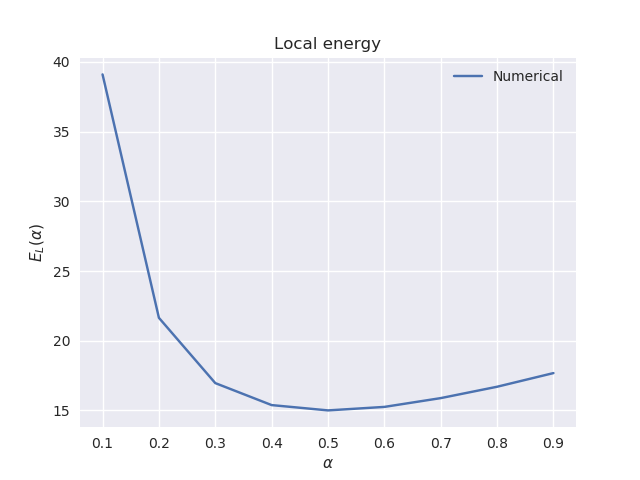
\includegraphics[scale=0.65]{images/energy.png}
    \caption{Add caption}
    \label{fig:energy}
\end{figure} 

\begin{figure} [H]
    \centering
    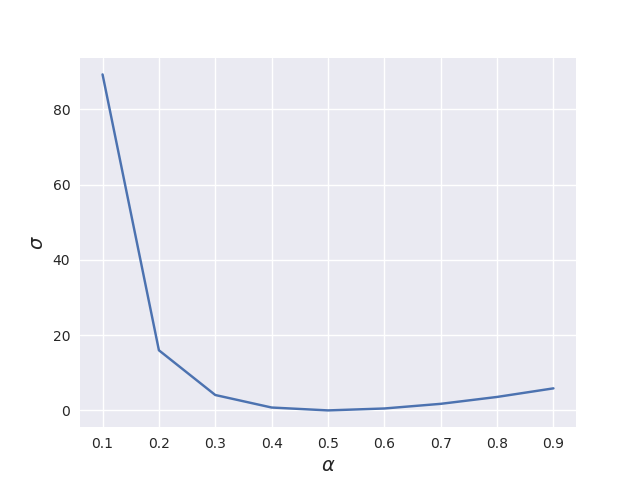
\includegraphics[scale=0.65]{images/variance.png}
    \caption{Add caption}
    \label{fig:variance}
\end{figure} 


\section{Discussion}

\section{Conclusion}

\end{document}
